\documentclass{beamer}

% PACKAGES
\usepackage[utf8]{inputenc}
\usepackage{graphicx}
\usepackage{booktabs}
\usepackage[slovak]{babel}
\usepackage{xcolor}
\usepackage{xurl}
\usepackage{times}
\usepackage{amssymb, amsmath}
\usepackage{bookmark}
\usepackage{listings}

% STYLES 
\usetheme{Madrid}
\renewcommand*{\lstlistingname}{Ukážka}
\definecolor{blue}{RGB}{0,0,255}

\lstset{
	basicstyle=\footnotesize,
	keywordstyle=\color{blue},
	language=pascal,
	morekeywords={is,endif,return},
	numbers=left,
	tabsize=4,
	xleftmargin=15pt,
	frame=single
}

% CONTENT

\title[ITY 5.~projekt]{\texorpdfstring{Typografie a~publikování\,--\,5.~projekt}}
\subtitle{Dátová štruktúra zásobník}

\author{Peter Zdravecký}

\institute[VUT FIT]
{
	Vysoké učení technické v~Brně\\
	Fakulta informačních technologií
}

\begin{document}

\maketitle

\begin{frame}
    \frametitle{Obsah}
    \tableofcontents
\end{frame}


\section{Úvod}
\begin{frame}{Úvod}
    Zásobník je jedna z najjednoduchších a najviac používaných dátových štruktúr.
    \medskip 
    \begin{itemize}
        \item Lineárna dátová štruktúra
        \item Princíp LIFO (Last in, First out), resp. FILO
        \item Implementácia \textbf{poľom}: k vrcholu sa pristupuje cez index
        \item Implementácia \textbf{lineárnym zoznamom}: k vrcholu sa pristupuje ukazateľom
    \end{itemize}

\end{frame}


\section{Základné operácie}
\begin{frame}{Základné operácie}
    Zoznam základných operácii, ktoré sa vykonávajú nad dátovou štruktúrou zásobník (implementácia poľom).
    \bigskip

    Základne operácie:
    \begin{itemize}
        \item \texttt{Push}\,--\,$O$(1)\,--\,Pridá položku do zásobníka. Ak je zásobník plný nastaví sa príznak pretečenia. 
        \item \texttt{Pop}\,--\,$O$(1)\,--\,Vyberie položku zo zásobníka. Ak je zásobník prázdny nastaví sa príznak podtečenia.
    \end{itemize}
    Dodatočné operácie:
\begin{itemize}
        \item \texttt{Top}\,--\,$O$(1)\,--\,Vráti položku ktorá sa nachádza na vrchole zásobníka.
        \item \texttt{isEmpty}\,--\,$O$(1)\,--\,Vráti \texttt{True} v prípade že zásobník je prázdny, ak nieje vráti sa \texttt{False}.
        \item \texttt{isFull}\,--\,$O$(1)\,--\,Vráti \texttt{True} v prípade že zásobník je plný, ak nieje vráti sa \texttt{False}.
\end{itemize}
\end{frame}


\section{Grafická ukážka}
\begin{frame}{Grafická ukážka}
    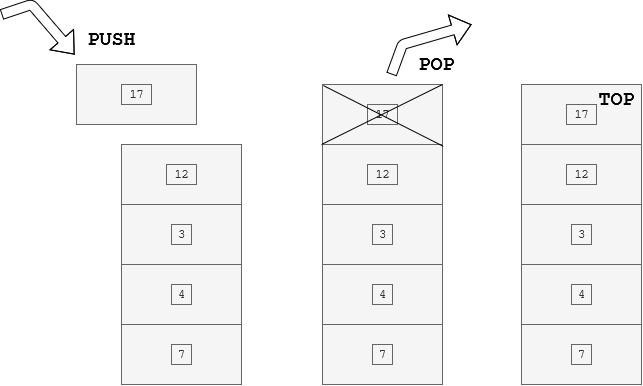
\includegraphics[scale=0.5]{example.png}
\end{frame}

\section{Pseudokód - PUSH}
\begin{frame}[fragile,c]{Pseudokód - PUSH}
    \begin{lstlisting}[caption=Procedúra PUSH nad dátovou štruktúrou zásobník,captionpos=b]
begin procedure push: stack, data

    if isFull(stack)
        return null
    endif
    
    top <- top + 1
    stack[top] <- data

end procedure
\end{lstlisting}
\end{frame}


\section{Pseudokód - POP}
\begin{frame}[fragile,c]{Pseudokód - POP}
\begin{lstlisting}[caption=Procedúra POP nad dátovou štruktúrou zásobník,captionpos=b]
begin procedure pop: stack, data

    if isEmpty(stack)
        return null
    endif
    
    data <- stack[top]
    top <- top - 1

end procedure
\end{lstlisting}
\end{frame}

\section{Využitie}
\begin{frame}{Využitie zásobníku v praxi}
    \begin{itemize}
        \item Syntaktická analýza
        \item Vyhodnocovanie matematických výrazov
        \item Konverzia výrazu napr.: infix do postfixu
        \item Správa pamäte
        \item Backtracking problémy
        \item Volanie funkcií
        \item Reverzia stringu
        \item Operácia \emph{undo}, napr. v textových editoroch
        \item Prehľadávanie stavového priestoru (Depth First Search)
        \item \dots
    \end{itemize}
\end{frame}


\section{Záver}
\begin{frame}{Záver}
    Zdroje:
    \begin{itemize}
        \item \url{https://en.wikipedia.org/wiki/Stack_(abstract_data_type)}
        \item \url{https://www.quora.com/What-are-the-real-life-applications-of-stack-data-structure}
        \item Študijné materiály predmetu IAL
    \end{itemize}
    \bigskip
    \centering{\huge{Ďakujem za pozornosť}}
\end{frame}

\end{document}
